\newif\ifsolutions
\solutionstrue % Show solutions
%\solutionsfalse % Hide solutions

\documentclass{article}
\usepackage{geometry}
\geometry{margin=1in}
\usepackage{tikz}
\usepackage{amssymb}

% fleqn allows setting indent of display math
\usepackage[fleqn]{amsmath}
\setlength{\mathindent}{0pt} % Set indent
% Disable equation numbering (https://tex.stackexchange.com/a/360378)
\makeatletter
\renewcommand\tagform@[1]{}
\makeatother

% Allow Unicode (some, e.g., © and £ at least)
% https://tex.stackexchange.com/questions/370278/is-there-any-reason-to-use-inputenc
\usepackage[utf8]{inputenc}

% Hyperlinks
\usepackage{hyperref}
\hypersetup{colorlinks=true, urlcolor=blue, linkcolor=blue}

% Prevent indentation of paragraphs
\setlength\parindent{0pt}
\setlength{\parskip}{\baselineskip}

% Spacing above/below equations
% https://tex.stackexchange.com/a/69678
\AtBeginDocument{%
 \abovedisplayskip=-\parskip
 \abovedisplayshortskip=-\parskip
 \belowdisplayskip=0pt
 \belowdisplayshortskip=0pt
}

% Allow 3 additional subsection levels
% https://tex.stackexchange.com/a/60212
\usepackage{titlesec}
\setcounter{secnumdepth}{6}
% H4 in HTML
\titleformat{\paragraph}{\normalfont\normalsize\bfseries}{\theparagraph}{1em}{}
\titlespacing*{\paragraph}{0pt}{3.25ex plus 1ex minus .2ex}{1.5ex plus .2ex}
% H5 in HTML
\titleformat{\subparagraph}{\normalfont\normalsize\bfseries}{\thesubparagraph}{1em}{}
\titlespacing*{\subparagraph}{0pt}{3.25ex plus 1ex minus .2ex}{1.5ex plus .2ex}
% H6 in HTML
\titleformat{\subsubparagraph}{\normalfont\normalsize\bfseries}{\thesubsubparagraph}{1em}{}
\titlespacing*{\subsubparagraph}{0pt}{3.25ex plus 1ex minus .2ex}{1.5ex plus .2ex}

% So enumerate at all levels is numbers
% https://tex.stackexchange.com/questions/78842/nested-enumeration-numbering
\renewcommand{\labelenumii}{\arabic{enumii}.}
\renewcommand{\labelenumiii}{\arabic{enumiii}.}
\renewcommand{\labelenumiv}{\arabic{enumiv}.}

\renewcommand{\mbox}{\text}
\newcommand{\ds}[0]{\displaystyle}
\newcommand{\ihat}[0]{\hat{\boldsymbol{\imath}}}
\newcommand{\jhat}[0]{\hat{\boldsymbol{\jmath}}}
\newcommand{\khat}[0]{\hat{\boldsymbol{k}}}
\newcommand{\xhat}[0]{\hat{\mathbf{x}}}
\newcommand{\yhat}[0]{\hat{\mathbf{y}}}
\newcommand{\zhat}[0]{\hat{\mathbf{z}}}
\newcommand{\rhat}[0]{\hat{\mathbf{r}}}
\newcommand{\bfvec}[1]{\vec{\mathbf{#1}}}
\newcommand{\bfcdot}[0]{\boldsymbol{\cdot}}

\usepackage{fancyhdr}
\pagestyle{fancy}
\lhead{Lorentz Force}
\rhead{\thepage}
\fancyfoot{}

\begin{document}

\section{Introduction}

A stationary or moving charge $q$ in an electric field (created by other charges) experiences a force of

\begin{equation}
\bfvec{F} = q\bfvec{E}
\end{equation}

A moving charge creates a magnetic field. A moving charge $q$ in a magnetic field (created by other moving charges) experiences a force of

\begin{equation}
\bfvec{F} = q\bfvec{v}\times\bfvec{B}
\end{equation}

The direction of the force on $q$ is perpendicular to a plane that contains $\bfvec{v}$ and $\bfvec{B}$. This plane can be visualized by imagining orienting a flat piece of paper such that both the  $\bfvec{v}$ and $\bfvec{B}$ vectors lie on the paper. The direction of $\bfvec{v}\times\bfvec{B}$ is perpendicular to the paper. As discussed in the Electric Flux activity, there are two perpendicular directions for a plane; the one to choose is determined by the right--hand rule for cross products.

The magnitude of $\bfvec{F}$ can be computed using the above equation to find $F_x$, $F_y$, and $F_z$ and then $F=\sqrt{F_x^2+F_y^2+F_z^2}$. Or, one can use

\begin{equation}
F = |q|vB\sin\phi\thinspace,
\end{equation}

where $\phi$ is the angle between $\bfvec{v}$ and $\bfvec{B}$ and $0 \le\phi \le 180^{\circ}$. (For example, the angle between two vectors can be said to be $\phi=10^{\circ}$ or $\phi=350^{\circ}$. In the above equation, use $10^{\circ}$; if $350^{\circ}$ was used, you would get a negative value for the magnitude of $F$, which is positive by definition because it is a magnitude.)

There are two special cases for which the general equation $\bfvec{F} = q\bfvec{v}\times\bfvec{B}$ simplifies to a very simple equation:

\begin{enumerate}

  \item If the direction of motion of $q$ is perpendicular to the magnetic field (so that $\phi = 90^{\circ}$), the magnitude of the force is $F = qvB$ and the direction of $F$ is determined by the right--hand rule.

  \item If the direction of motion is parallel or antiparallel to the magnetic field (so that $\phi = 0^{\circ}$ or $\phi = 180^{\circ}$), the magnitude of the force is zero.

\end{enumerate}

When the vectors in a cross product are both in a Cartesian coordinate plane (so that the angle $\phi$ between them is easily computed), the formula $F = |q|vB\sin\phi$ can be used to find the magnitude of $F$ and its direction is given by the right--hand rule. Otherwise, finding the angle $\phi$ and the perpendicular direction requires a diagram and several steps of trigonometry. In this case, using vector notation to compute $\bfvec{F}$ is easier.

\newpage

\section{Calculating Forces}

In this section, you will compute the magnitude and direction of the force in two ways: 1. using $F = |q|vB\sin\phi$ and the cross--product right--hand rule and 2. using vector notation to find $\bfvec{F}=q\bfvec{v}\times\bfvec{B}$ in component form and then computing the magnitude $|\bfvec{F}|$. 

The problems given are most easily solved using the first method. You are also asked to solve the problems using the second method as preparation for problems that are more easily solved this way.

\subsection{Computing $\bfvec{F}$ and $F$ Using Vector Notation}

The calculation of the cross product when both vectors in the cross product are along one of the Cartesian coordinate axes is the easiest case (e.g.,  $\bfvec{v}=v_o\jhat$ and $\bfvec{B}=B_o\ihat$). There are two ways of determining the cross--product $\bfvec{v}\times\bfvec{B}$ in this case:

\begin{enumerate}

  \item using the right--hand rule with the two unit vectors to determine the direction of $\bfvec{F}$ and $|q|vB$ for the magnitude of $F$ or

  \item using $q\bfvec{v}\times\bfvec{B}$ and the following table of cross products.

        \begin{equation}
        \begin{align*}
        \ihat\times\ihat &  = 0  & \jhat\times\jhat & =0  &   \khat\times\khat & = 0 \\
        \ihat\times\jhat & = \khat  & \jhat\times\khat & = \ihat  & \khat\times\ihat & =  \jhat \\
        \jhat\times\ihat & =-\khat & \khat\times\jhat &  = -\ihat & \ihat\times\khat & = -\jhat \\
        \end{align*}
        \end{equation}

\end{enumerate}

There is a mnemonic (memory) device for remembering this table. Suppose you do the cross product of two consecutive unit vectors in the order indicated by the arrows in the circle shown in the following figure. In that case, the result is the remaining unit vector (the second row in the table). If you do the cross product of two unit vectors in reverse order, the result is the remaining unit vector with a negative sign (the third row in the table).



\tikzset{every picture/.style={line width=0.75pt}} %set default line width to 0.75pt        

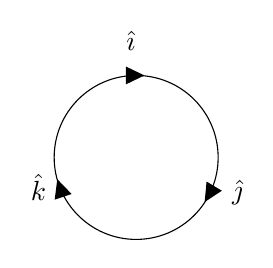
\begin{tikzpicture}[x=0.75pt,y=0.75pt,yscale=-1,xscale=1]
%uncomment if require: \path (0,119); %set diagram left start at 0, and has height of 119

%Shape: Circle [id:dp5988157550687865] 
\draw   (25.5,65.65) .. controls (25.5,43.83) and (43.18,26.15) .. (65,26.15) .. controls (86.82,26.15) and (104.5,43.83) .. (104.5,65.65) .. controls (104.5,87.47) and (86.82,105.15) .. (65,105.15) .. controls (43.18,105.15) and (25.5,87.47) .. (25.5,65.65) -- cycle ;
%Straight Lines [id:da42189417649788785] 
\draw    (29,82.14) -- (27.95,78.99) ;
\draw [shift={(27,76.14)}, rotate = 71.57] [fill={rgb, 255:red, 0; green, 0; blue, 0 }  ][line width=0.08]  [draw opacity=0] (8.93,-4.29) -- (0,0) -- (8.93,4.29) -- cycle    ;

%Straight Lines [id:da47415096212675123] 
\draw    (67,26.15) ;
\draw [shift={(69,26.15)}, rotate = 180] [fill={rgb, 255:red, 0; green, 0; blue, 0 }  ][line width=0.08]  [draw opacity=0] (8.93,-4.29) -- (0,0) -- (8.93,4.29) -- cycle    ;
%Straight Lines [id:da10747602373995879] 
\draw    (101,82.15) -- (99.54,84.57) ;
\draw [shift={(98,87.14)}, rotate = 300.99] [fill={rgb, 255:red, 0; green, 0; blue, 0 }  ][line width=0.08]  [draw opacity=0] (8.93,-4.29) -- (0,0) -- (8.93,4.29) -- cycle    ;


% Text Node
\draw (13,72.4) node [anchor=north west][inner sep=0.75pt]    {$\hat{k}$};
% Text Node
\draw (110,75.4) node [anchor=north west][inner sep=0.75pt]    {$\hat{\jmath }$};
% Text Node
\draw (59,3.4) node [anchor=north west][inner sep=0.75pt]    {$\hat{\imath }$};


\end{tikzpicture}


\ifsolutions\else
\newpage
\fi

\subsection{Example}

In the following diagram, a positive charge $q$ moves with a velocity in a region of space with a magnetic field.



\tikzset{every picture/.style={line width=0.75pt}} %set default line width to 0.75pt        

\begin{tikzpicture}[x=0.75pt,y=0.75pt,yscale=-1,xscale=1]
%uncomment if require: \path (0,150); %set diagram left start at 0, and has height of 150

%Straight Lines [id:da4740594144334427] 
\draw    (23,54.14) -- (23,24.5) ;
\draw [shift={(23,21.5)}, rotate = 90] [fill={rgb, 255:red, 0; green, 0; blue, 0 }  ][line width=0.08]  [draw opacity=0] (8.93,-4.29) -- (0,0) -- (8.93,4.29) -- cycle    ;
%Straight Lines [id:da3530708515027745] 
\draw    (175.5,25.5) -- (175.5,51) ;
\draw [shift={(175.5,54)}, rotate = 270] [fill={rgb, 255:red, 0; green, 0; blue, 0 }  ][line width=0.08]  [draw opacity=0] (8.93,-4.29) -- (0,0) -- (8.93,4.29) -- cycle    ;
%Straight Lines [id:da8793619583100336] 
\draw    (361.5,54.14) -- (333.36,54.14) ;
\draw [shift={(330.36,54.14)}, rotate = 360] [fill={rgb, 255:red, 0; green, 0; blue, 0 }  ][line width=0.08]  [draw opacity=0] (8.93,-4.29) -- (0,0) -- (8.93,4.29) -- cycle    ;
%Straight Lines [id:da22154182372047826] 
\draw    (32.5,124) -- (61.5,124.45) ;
\draw [shift={(64.5,124.5)}, rotate = 180.9] [fill={rgb, 255:red, 0; green, 0; blue, 0 }  ][line width=0.08]  [draw opacity=0] (8.93,-4.29) -- (0,0) -- (8.93,4.29) -- cycle    ;
%Shape: Axis 2D [id:dp581121235433776] 
\draw  (440.93,34.5) -- (465.31,34.5)(443.37,14.42) -- (443.37,36.73) (458.31,29.5) -- (465.31,34.5) -- (458.31,39.5) (438.37,21.42) -- (443.37,14.42) -- (448.37,21.42)  ;
\draw   ;

%Straight Lines [id:da32647207661620703] 
\draw    (53,55) -- (85,55) ;
\draw [shift={(87,55)}, rotate = 180] [color={rgb, 255:red, 0; green, 0; blue, 0 }  ][line width=0.75]    (10.93,-3.29) .. controls (6.95,-1.4) and (3.31,-0.3) .. (0,0) .. controls (3.31,0.3) and (6.95,1.4) .. (10.93,3.29)   ;

%Straight Lines [id:da06082950450537594] 
\draw    (205,53) -- (237,53) ;
\draw [shift={(239,53)}, rotate = 180] [color={rgb, 255:red, 0; green, 0; blue, 0 }  ][line width=0.75]    (10.93,-3.29) .. controls (6.95,-1.4) and (3.31,-0.3) .. (0,0) .. controls (3.31,0.3) and (6.95,1.4) .. (10.93,3.29)   ;

%Straight Lines [id:da9631975494507745] 
\draw    (371,54) -- (403,54) ;
\draw [shift={(405,54)}, rotate = 180] [color={rgb, 255:red, 0; green, 0; blue, 0 }  ][line width=0.75]    (10.93,-3.29) .. controls (6.95,-1.4) and (3.31,-0.3) .. (0,0) .. controls (3.31,0.3) and (6.95,1.4) .. (10.93,3.29)   ;

%Straight Lines [id:da4542851964533421] 
\draw    (71,125) -- (103,125) ;
\draw [shift={(105,125)}, rotate = 180] [color={rgb, 255:red, 0; green, 0; blue, 0 }  ][line width=0.75]    (10.93,-3.29) .. controls (6.95,-1.4) and (3.31,-0.3) .. (0,0) .. controls (3.31,0.3) and (6.95,1.4) .. (10.93,3.29)   ;

%Straight Lines [id:da572318859075251] 
\draw    (201,125) -- (233,125) ;
\draw [shift={(235,125)}, rotate = 180] [color={rgb, 255:red, 0; green, 0; blue, 0 }  ][line width=0.75]    (10.93,-3.29) .. controls (6.95,-1.4) and (3.31,-0.3) .. (0,0) .. controls (3.31,0.3) and (6.95,1.4) .. (10.93,3.29)   ;

%Straight Lines [id:da9113860846395712] 
\draw    (341,124) -- (373,124) ;
\draw [shift={(375,124)}, rotate = 180] [color={rgb, 255:red, 0; green, 0; blue, 0 }  ][line width=0.75]    (10.93,-3.29) .. controls (6.95,-1.4) and (3.31,-0.3) .. (0,0) .. controls (3.31,0.3) and (6.95,1.4) .. (10.93,3.29)   ;


% Text Node
\draw (285,42.14) node [anchor=north west][inner sep=0.75pt]   [align=left] {c.};
% Text Node
\draw (150,115.14) node [anchor=north west][inner sep=0.75pt]   [align=left] {e.};
% Text Node
\draw (288,118.14) node [anchor=north west][inner sep=0.75pt]   [align=left] {f.};
% Text Node
\draw (180,115.6) node [anchor=north west][inner sep=0.75pt]    {$\odot $};
% Text Node
\draw (317,115.6) node [anchor=north west][inner sep=0.75pt]    {$\otimes $};
% Text Node
\draw (18,0.4) node [anchor=north west][inner sep=0.75pt]    {$\mathbf{v}$};
% Text Node
\draw (169,5.4) node [anchor=north west][inner sep=0.75pt]    {$\mathbf{v}$};
% Text Node
\draw (313,44.4) node [anchor=north west][inner sep=0.75pt]    {$\mathbf{v}$};
% Text Node
\draw (19,113.4) node [anchor=north west][inner sep=0.75pt]    {$\mathbf{v}$};
% Text Node
\draw (171,114.4) node [anchor=north west][inner sep=0.75pt]    {$\mathbf{v}$};
% Text Node
\draw (308,115.4) node [anchor=north west][inner sep=0.75pt]    {$\mathbf{v}$};
% Text Node
\draw (380,115.4) node [anchor=north west][inner sep=0.75pt]    {$\mathbf{B}$};
% Text Node
\draw (240,116.4) node [anchor=north west][inner sep=0.75pt]    {$\mathbf{B}$};
% Text Node
\draw (110,116.4) node [anchor=north west][inner sep=0.75pt]    {$\mathbf{B}$};
% Text Node
\draw (410,45.4) node [anchor=north west][inner sep=0.75pt]    {$\mathbf{B}$};
% Text Node
\draw (244,44.4) node [anchor=north west][inner sep=0.75pt]    {$\mathbf{B}$};
% Text Node
\draw (92,46.4) node [anchor=north west][inner sep=0.75pt]    {$\mathbf{B}$};
% Text Node
\draw (444.48,0.16) node [anchor=north west][inner sep=0.75pt]  [font=\scriptsize]  {$y$};
% Text Node
\draw (467.01,28.17) node [anchor=north west][inner sep=0.75pt]  [font=\scriptsize]  {$x$};
% Text Node
\draw (2,113.14) node [anchor=north west][inner sep=0.75pt]   [align=left] {d.};
% Text Node
\draw (148,35.14) node [anchor=north west][inner sep=0.75pt]   [align=left] {b.};
% Text Node
\draw (1,42.14) node [anchor=north west][inner sep=0.75pt]   [align=left] {a.};


\end{tikzpicture}


For case f. in the figure above,

\begin{enumerate}

  \item Write a vector equation for both $\bfvec{v}$ and $\bfvec{B}$ and use it to compute the force vector using $\bfvec{F} = q\bfvec{v}\times\bfvec{B}$ assuming that $\bfvec{B}=B_o\ihat$ and $|\bfvec{v}|=v_o$. Then compute the magnitude of $\bfvec{F}$.

  \item Use $F = |q|vB\sin\phi$ to compute the magnitude of the force and use the right-hand rule to determine its direction.

\end{enumerate}

\textbf{Answer}

\textbf{f.1}

$\bfvec{v}=-v_o\khat$, so $\bfvec{F} = q(-v_o\khat)\times (B_o\ihat)=-qv_oB_o(\khat\times \ihat)=-qv_oB_o\jhat$;

$|\bfvec{F}|=|-qv_oB_o\jhat| = |-qv_oB_o||\jhat|=|q|v_oB_o$.

\textbf{f.2}

$\phi=90^{\circ}$, so $F = |q|v_oB_o\sin(90^{\circ})=|q|v_oB_o$.

The right--hand rule gives direction as $-\jhat$.

\subsection{Problem}

Answer questions 1. and 2. given in the previous problem for cases a.--e. in the figure above. Assume that the magnitude of the velocity is $v_o$ and the magnitude of the magnetic field is $B_o$.

{\bf a.1}

\ifsolutions
$\bfvec{v}=v_o\jhat$, so $\bfvec{F} = q,(v_o\jhat)\times (B_o\ihat)=qv_oB_o(\jhat\times \ihat)=-qv_oB_o\khat$; $|\bfvec{F}|=qv_oB_o$
\else

\vskip 48pt
\fi
\ifsolutions\else
\vskip 48pt
\fi

{\bf a.2}

\ifsolutions
$\phi=90^{\circ}$, so $F = qv_oB_o\sin(90^{\circ})=qv_oB_o$.
\fi

{\bf b.1}

\ifsolutions
$\bfvec{v}=-v_o\jhat$, so $\bfvec{F} = -q,(v_o\jhat)\times (B_o\ihat)=qv_oB_o(\jhat\times \ihat)=qv_oB_o\khat$; $|\bfvec{F}|=qv_oB_o$
\else

\vskip 48pt
\fi
\ifsolutions\else
\vskip 48pt
\fi
{\bf b.2}
\ifsolutions
$\phi=90^{\circ}$, so $F = qv_oB_o\sin(90^{\circ})=qv_oB_o$.
\else

\vskip 48pt
\fi
\ifsolutions\else
\vskip 48pt
\fi

{\bf c.1}

\ifsolutions
$\bfvec{v}=-v_o\ihat$, so $\bfvec{F} = -q(v_o\ihat)\times (B_o\ihat)=-qv_oB_o(\jhat\times \ihat)=0$; $|\bfvec{F}|=0$
\else

\vskip 48pt
\fi
\ifsolutions\else
\vskip 48pt
\fi

{\bf c.2}

\ifsolutions
$\phi=90^{\circ}$, so $F = qv_oB_o\sin(180^{\circ})=0$.
\else

\vskip 48pt
\fi
\ifsolutions\else
\vskip 48pt
\fi

{\bf d.1}

\ifsolutions
$\bfvec{v}=v_o\ihat$, so $\bfvec{F} = q(v_o\ihat)\times (B_o\ihat)=qv_oB_o(\ihat\times \ihat)=0$; $|\bfvec{F}|=0$
\else

\vskip 48pt
\fi
\ifsolutions\else
\vskip 48pt
\fi

{\bf d.2}

\ifsolutions
$\phi=90^{\circ}$, so $F = qv_oB_o\sin(0^{\circ})=0$.
\else

\vskip 48pt
\fi
\ifsolutions\else
\vskip 48pt
\fi

{\bf e.1}

\ifsolutions
$\bfvec{v}=v_o\khat$, so $\bfvec{F} = q,(v_o\khat)\times (B_o\ihat)=qv_oB_o(\khat\times \ihat)=qv_oB_o\jhat$; $|\bfvec{F}|=qv_oB_o$
\else

\vskip 48pt
\fi
\ifsolutions\else
\vskip 48pt
\fi

{\bf e.2}

\ifsolutions
$\phi=90^{\circ}$, so $F = qv_oB_o\sin(90^{\circ})=qv_oB_o$.
\else

\newpage
\fi
\ifsolutions\else
\newpage
\fi

\section{Trajectories}

If the magnetic force on a charge particle is not zero the direction of its velocity vector will change. Because the magnetic force depends on the velocity vector direction, the magnetic force vector will also change.

For a charged particle moving in a region of space with a constant magnetic field (both in magnitude and direction), there are three general trajectories:

\begin{enumerate}

  \item If the velocity is parallel to the magnetic field lines, the trajectory is a straight line because no magnetic forces are acting on it.

  \item If velocity is perpendicular to the magnetic field lines, the trajectory is spiral. The particle rotates in a circle in the same plane as the velocity vector and drifts parallel or antiparallel to the field lines.

  \item The velocity has parallel and perpendicular components to the magnetic field line. In this case, the particle will move at a constant speed parallel or antiparallel to the field lines and in a circle around the field line. The trajectory is a spiral.

\end{enumerate}

\subsection{Problem}

Use the simulation at https://ophysics.com/em8.html to verify the above three statements. State the settings that you used to create the trajectory. Also, state how the settings affected the trajectory and in which way (for example, for case $a.$, ``changing $m$ did not change the shape of the type or shape of the trajectory"). 

1.

2.

3.

\ifsolutions\else
\newpage
\fi

\subsection{Problem}

Consider the following cases and describe the trajectory of the particle in words in the table below (e.g., ``circle in $x$--$y$ plane; ccw when viewed from a point on $+z$ axis" or ``spiral with motion in $+z$ direction; ccw when viewed from a point on $+z$ axis"). You may use the simulation to check some of your answers. 

\ifsolutions
{\bf Answer:} I determine the direction of rotation by using a right-hand rule -- wrap fingers around $\mathbf{B}$, and the direction of motion of a $+$ charge is in the opposite direction of my fingers. You'll learn later that this rule tells you that the magnetic field created by the charge that rotates around the magnetic field is in the opposite direction of the magnetic field that caused it to rotate.

Another way of doing this is drawing the $\mathbf{B}$ and $\mathbf{v}$ vectors and determining the direction of force - the trajectory will be a circle with the rotation direction that is required to rotate the velocity vector towards the force vector.

For both cases, I draw an $x$, $y$, $z$ axis, and the vectors $\mathbf{B}$, $\mathbf{v}$, and $\mathbf{F}$.

a. $\mathbf{B} =  B_o\hat{\mathbf{x}}$  $\mathbf{v} = v_o\hat{\mathbf{x}}$: Trajectory is straight line along $\hat{\mathbf{x}}$ direction.

b. $\mathbf{B} =  B_o\hat{\mathbf{z}}$ $\mathbf{v} = v_o\hat{\mathbf{x}}$: Trajectory is cw circle in $x$--$y$ plane when viewed from point on $+z$ axis

c. $\mathbf{B} = -B_o\hat{\mathbf{y}}$ $\mathbf{v} = v_o\hat{\mathbf{z}}$: Trajectory is ccw circle in $x$--$z$ plane when viewed from point on $+y$ axis

d. $\mathbf{B} = B_o\hat{\mathbf{x}} $ $\mathbf{v} = v_o\hat{\mathbf{x}}+v_o\hat{\mathbf{y}}$: Trajectory is cw circle in $y$--$z$ plane when viewed from point on the $+x$ axis. Spiral growing in +x direction.

e. $\mathbf{B} = -B_o\hat{\mathbf{y}}$ $\mathbf{v} = v_o\hat{\mathbf{y}}+v_o\hat{\mathbf{z}}$: Trajectory is ccw circle in $x$--$y$ plane when viewed from point on $+y$ axis. Spiral growing in $+y$ direction.
\else
\begin{equation}
\begin{align*}
a.\quad & \mathbf{B} =  B_o\hat{\mathbf{x}}&  \mathbf{v} &= v_o\hat{\mathbf{x}} & & \bf{Trajectory =} \\\\\\\\ \\\\
b.\quad & \mathbf{B} =  B_o\hat{\mathbf{z}} &  \mathbf{v} & = v_o\hat{\mathbf{x}}& &  \bf{Trajectory =} \\\\\\\\ \\\\
c.\quad  & \mathbf{B} = -B_o\hat{\mathbf{y}} & \mathbf{v} & = v_o\hat{\mathbf{z}}& & \bf{Trajectory =} \\\\\\\\ \\\\
d.\quad  & \mathbf{B} = B_o\hat{\mathbf{x}} & \mathbf{v} & = v_o\hat{\mathbf{x}}+v_o\hat{\mathbf{y}}& &\bf{Trajectory =}\\\\\\\\ \\\\
e.\quad  & \mathbf{B} = -B_o\hat{\mathbf{y}} & \mathbf{v} & = v_o\hat{\mathbf{y}}+v_o\hat{\mathbf{z}}& & \bf{Trajectory =} & 
\end{align*}
\end{equation}
\fi
\ifsolutions\else
\begin{equation}
\begin{align*}
a.\quad & \mathbf{B} =  B_o\hat{\mathbf{x}}&  \mathbf{v} &= v_o\hat{\mathbf{x}} & & \bf{Trajectory =} \\\\\\\\ \\\\
b.\quad & \mathbf{B} =  B_o\hat{\mathbf{z}} &  \mathbf{v} & = v_o\hat{\mathbf{x}}& &  \bf{Trajectory =} \\\\\\\\ \\\\
c.\quad  & \mathbf{B} = -B_o\hat{\mathbf{y}} & \mathbf{v} & = v_o\hat{\mathbf{z}}& & \bf{Trajectory =} \\\\\\\\ \\\\
d.\quad  & \mathbf{B} = B_o\hat{\mathbf{x}} & \mathbf{v} & = v_o\hat{\mathbf{x}}+v_o\hat{\mathbf{y}}& &\bf{Trajectory =}\\\\\\\\ \\\\
e.\quad  & \mathbf{B} = -B_o\hat{\mathbf{y}} & \mathbf{v} & = v_o\hat{\mathbf{y}}+v_o\hat{\mathbf{z}}& & \bf{Trajectory =} & 
\end{align*}
\end{equation}
\fi

\end{document}